\section{Introduction}

There are tremendous amount of user-generated contents about medical information through the internet. As a result, there is a growing need for enriching medical-related knowledge, for which it can be very valuable for several tasks, such as medical document retrieval, medical question answering, and health-related text mining applications. However, understanding those various health-related contents, especially from social media, is simply not a trivial task since they are written in free text format (i.e. unstructured format), and often prone to grammatical and typographical glitches. Therefore, reducing the complex characteristics of the textual contents, including but not limited to linguistic variations, into structured information could be very beneficial for the text interpretation process. 

One possible solution is to extract medical terms that represents the document they belong to. The common approach is harnessing medical entity recognizer. However, we argue that there are many missing pieces of information when we merely rely on medical entities or terminologies as our main information for representing a particular document. In this paper, we present new keyphrases extraction techniques to extract more important information about the concept expressed inside the document. Furthermore, we also propose a new definition of keyphrases, which is based on our observation of health-related documents. Actually, our final goal is to develop medical question answering systems to assist physicians or people obtaining health information. The work presented in this paper is absolutely inline with our goal, since important keyphrases of a question document can be used to formulate a query for the passage retrieval subsystem. 

Keyphrases are usually selected phrases or clauses that can capture the main topic of a given document \cite{turney2000learning}. They can provide readers with highly valuable and representative information, such that looking at keyphrases is sufficient to understand the whole body of document. Moreover, keyphrases are important for text summarization, document clustering, and classification task (\cite{classDocumentEkp1}; \cite{qaEkp}; \cite{gong2009improving}). Previous works have shown that using keyphrases to generate queries can improve the quality of question retrieval in medical question answering forum \cite{cao2010automatically}.


Keyphrase extraction methods have been mostly using statistical approach (\cite{sparck1972statistical} \cite{zhang2007comparative} \cite{rake} \cite{mihalcea2004textrank}) and supervised learning approach (\cite{witten1999kea} \cite{medelyan2009human} \cite{marujoMAUI}). The statistical approach often involves keyword candidate selection and candidate's property calculation. The "keywordness" value of a candidate phrase is usually scored based on its typical length as well as frequency in which document it appears \cite{rake}. While the statistical approach is very efficient to generate keyphrases, our experiments showed that it performs poorly on user generated contents and short documents. The other approach is based on supervised learning, there are two common approach in supervised learning: classification and sequence labeling. In classification approach, candidate keyphrases are extracted using statistical \cite{sparck1972statistical} or language model \cite{ekpNeuralNetworks}. Then, the candidate keyphrases are classified whether a candidate is a keyphrase or not by using a pretrained model. However, classification approach cannot capture semantic relationship between words in a document \cite{surveyPopulerTerbaruEkp}.  In sequence labeling approach,  like the one proposed by \cite{cao2010automatically} and \cite{zhang2008automatic}. They define keyphrase extraction task as a sequence labeling task, in which each word in the document can have two possible labels: keyword or non-keyword. The method they proposed worked well by outperforming unsupervised approach. However, synonym and ambiguity words cannot be handled properly \cite{zhang2008automatic}.

In our work, we use the same approach as \cite{cao2010automatically} which treats keyphrase extraction as a sequence labeling task. In our experiment, we employed and combined various deep learning architectures, such as convolutional neural networks and bi-directional long short-term memory networks, to exploit high level features between neighboring word positions. To improve the quality of our model, we leverage several new hand-crafted features that can handle our keyphrase extraction problems in medical user-generated content, such as word importance and word stickiness features. The word importance feature is enable to rank words in a document by their importance value. The more important a word is to the content of document, the higher its "keywordness" value would seem to be. In addition, we also propose word stickiness feature to make our model constructs keyphrases better. 

We also employed pre-trained word embedding to incorporate contextual, semantic, and syntactic information of a word. For example, we found that pre-trained word embedding can handle slang words and abbreviations by giving their word vectors closer to the vectors of their canonical forms. Finally, to evaluate the effectiveness of our model, we collected and manually annotated data from Indonesian medical forum questions, such as alodokter, health detik, doktergratis, dokter.id, doktersehat, klikdokter \footnote{www.alodokter.com, health.detik.com, www.dokter.id, www.doktersehat.com, www.klikdokter.com}. After that, the dataset was used for both training and testing our computational models. For our baseline, we use RAKE  \cite{rake}, which is the current state of the art model for extracting keyphrases.


This paper is organized as follows.  In section 2 we discuss related works in keyphrase extraction. In section 3, the proposed keyphrase extraction method has been discussed. We present the evaluation and the experimental results in section 4. 

\section{Related Works}
In general, keyphrase extraction methods can be divided into two groups: unsupervised ranking (statistical) approach and supervised machine learning approach. For the unsupervised line of research, keyphrase extraction is formulated as a ranking problem, in which each candidate keyphrase is assigned a score that represents its keywordness value. Furthermore, this kind of approach does not require training data, which is often very difficult to obtain. On the other hand, supervised machine learning approach requires training data that contains a collection of documents with their labeled keywords. Using this approach, keyphrase extraction is usually treated as a classification or sequence labeling task in the level of words or phrases. The first step of this approach generates candidate keyphrases from a particular document. Finally, every candidate keyphrase in the document will be classified as either a keyphrase or non-keyphrase. Recently, a well-known supervised approach for keyphrase extraction is based on sequence labeling problem (\cite{zhang2008automatic}\cite{cao2010automatically}\cite{zhang2016keyphrase}). The assumption behind this model is that the decision on whether a particular word serves as a keyword is affected by the information from its neighboring word positions.

In the work of \cite{sparck1972statistical}, they leverage TF-IDF to get the most significant words. Specifically, they utilize term frequency and the inverse of document frequency to rank terms in the document. First, this Rapid Automatic Keywords Extraction \cite{rake} uses stopwords to split a document into several candidate keyphrases. All candidates will be ranked by the degrees and frequencies of all words inside them. Finally, the rank points of each candidate is obtained by summing over all degrees and frequencies of all words contained in each keyphrase. RAKE is proven to be successful for extracting keyphrases in special documents such as paper and article \cite{rake}.

There is also a popular graph-based approach, namely TextRank (U), i.e., a modified PageRank algorithm to extract keyphrases from a document. They exploit word co-occurrence information to build a document graph, in which a word serves as a node and co-occurence information determines an edge between two nodes (words). After they build the graph, they actually run PageRank algorithm to determine the keywordness score for each node in the graph. A word with high PageRank value denotes that its related concept can be found in many location inside the document, which means that it is a good candidate for keyword. After that, keyphrases can be obtained using post-processing step that may combine contiguous candidates into one keyphrase.

One of the earlier supervised approaches in the problem of keyphrase extraction is KEA \cite{witten1999kea}. KEA uses tf-idf and first occurrence of the term to identify candidate keyphrases. They use a machine-learning algorithm (i.e., Naive Bayes) to predict whether or not a candidate is a good keyphrase. \cite{medelyan2009human} developed a system called MAUI that can extract keyphrases using trained corpus and controlled vocabulary. MAUI itself is an improvement to the aforementioned supervised model, KEA. Furthermore, \cite{marujoMAUI} use word embedding and brown clustering as features. Their experiment result had shown that the proposed features and MAUI performs better than statistical methods, such as simple tf-idf approach.

The utilization of neural networks is also quite popular in the recent years. \cite{ekpNeuralNetworks} uses Feed Forward Neural Networks to classify candidate keyphrases. To extract candidate keyphrases, they use POS tag information for classifying all words in the document. Then, Deterministic Finite Automation (DFA) is used to extract noun phrases as candidate keyphrases. Furthermore, deep neural networks is also employed for extracting keyphrase, like the one proposed by \cite{zhang2016keyphrase}, that uses joint Recurrent Neural Networks (RNNs) layer to capture keyphrase sequences in microblogs. The research had shown that RNN is very effective to extract keyword.

Unfortunately, there are limited works regarding the task of keyphrase extraction in medical domain. \cite{ekpMedicalDocumentHybrid} use a hybrid medical knowledge base and statistical approach to extract keyphrases from medical articles. They use stopwords to split candidate keyphrases, then candidates are ranked with two aspects: PF-IDF (Phrase Frequency * Inverse Document Frequency) and domain knowledge which is extracted from medical article. In terms of medical social media content, \cite{cao2010automatically} use Conditional Random Fields (CRFs) for extracting keywords from medical questions in online health-forum. They use information, such as word location and length as features in their experiments.

\section{METHODOLOGY}
\subsection{DATA AND ANNOTATION}
To analyze the effectiveness of our model for keyphrase extraction in user-generated medical domain, we constructed an evaluation dataset. A a number of questions was gathered from Indonesian medical question answering forum. The data was crawled by \cite{skripsiKakRadit} and \cite{skripsiWahid} in their experiment. Generally, we gathered 416 question-answer pairs from \cite{skripsiKakRadit} and \cite{skripsiWahid}. We decided to use the same question-answers pairs to observe our keyphrases and medical entities that has been annotated by them. In addition, system for recognizing medical entities is not fully build, by using the same document we can use the annotated medical entities as our feature.

From analyzing these question-answer pairs, we found some noise and unnecessary information. Question and answer have different main topic and focus. Moreover, we are focusing our task for getting user intentions and needs in our experiment. Based on that problem, we only use questions by users and remove answers by the doctors because it would be a better representation of user intentions and needs. There is also unnecessary information such as URL and email. We replace URL with “URL”  and email with “email” since we were focusing on textual content. Moreover, we also removed ads and spam in the data we gathered.

Because we want to process all the questions by users, we tokenize every question in our data. The tokenization process included separating alphanumeric with non-alphanumeric. Then separating alphanumeric with numeric. 

To evaluate the quality of our model. We manually annotated or data to label keyphrases in 416 questions. In this work, we use "IOB" tagging scheme to label every word \cite{collobert2011natural}. In Table X, we give an example sequence with labels for each word. The statistical information of the dataset can be seen in Table X
\begin{table}
	\caption{Statistical information of dataset. W, K, $\bar{N}_{w}$, $\bar{N}_{k}$ are the total of words, number of keyphrases, average number of words, and average number of keyphrases in each question, respectively.}
	\label{tab:descriptive_stats}
	\begin{tabular}{lcccc}
		\toprule
		#questions&W&K&$\bar{N}_{w}$&$\bar{N}_{k}$\\
		\midrule
		416 & 26747  & 64.76 & 1861 & 4.49 \\
		
		\bottomrule
	\end{tabular}
\end{table}
\subsection{TASK DEFINITIONS}
\subsection{MODEL ARCHITECTURE}
We process the sequences word by word. Features are extracted from every word as the input representation of the model. The output for this words are label which describe a word is either part of keyphrase or not.

To give our model a better insight of context, we introduce Convolutional Neural Networks (CNNs) to capture context from three adjacent words.  From our observation, to know whether a word is part of keyphrase or not, we need to know the context of the word itself. For example, “Doc, i have a frequent back pain. What happen?”. The keyphrase for previous example is “frequent back pain”. In order to know that “back” is part of keyphrase, we need information from the word “frequent” which give an intensity of a symptom and “pain” which refer to “back pain” as main term. With CNNs, we argue that our model can capture the surrounding information of a word.

To get a better inference, information from the past and future sequences can be integrated. This approach is proven effective  in sequence labeling task such as semantic role labeling \cite{SMRzhou2015end} and named entity recognition \cite{ma2016end}. Hence, we utilized  bi-directional LSTM (B-LSTM) for extracting structural knowledge by processing sequences both forward and backward.
To perform the sequence tagging task, we build a fully connected layer in the top of our model. This layer will classify the output of our model with softmax activation function.

We also experimented on customizing the way we input the features underneath our aforementioned networks. Instead of concatenating all feature into one vector, we tried to give weight for every feature we have. We argue that each feature have different contribution to the model. In order to do so, we create a new layer underneath our model to do the weighting scenario. The following equation to weight all feature can be seen in below:
\begin{equation}
	Z =  tanh(W _{1}*F_{1} + W_{2}*F_{2} + .. + W_{n}*F_{n})
\end{equation}
Where $W_{i}$ are the weight for each feature and $F_{i}$ are the extracted feature in vector form.
\section{EXPERIMENTS}
In this section, we analyzed the importance of our features by conducting a feature ablation study. Furthermore, we also established a scenario to test the performance of our model.
\subsection{Feature Ablation Study}
In this part, perform a feature ablation study. By considering all the features, and then removing one of these features, we want to estimate the importance of the features. To the experiment. We use 80\% as training set, and 20\% as a testing set. We used precision (P), recall (R), and F1-score (F1) as evaluation metrics. Table \ref{tab:ablation} show the experimental result. Then, we use LSTM as evaluation model because it is the most simple architecture. These are the following features we proposed: word stickiness (Ws), word abbreviation and acronym (Wa), Medical Entities (Me), Word Location (Wp), Word Length (Wl), Word Importance (Wi), POS tag (Pt), Medical Dictionary (Md).

\begin{table*}
	\caption{Feature Ablation Study Result}
	\label{tab:ablation}
	\begin{tabular}{lccc}
		\toprule
		Features&Precision&Recall&F-Measure\\
		\midrule
			We + Ws + Wa + Me + Wp + Wl + Wi + Pt + Md & 79.93\% & 57.45\% & 66.85\% \\
			
			Ws + Wa + Me + Wp + Wl + Wi + Pt + Md & 84.01\% & 75.79\% & 79.69\% \\
			
			We + Wa + Me + Wp + Wl + Wi + Pt + Md & 76.39\% & 73.59\% & 74.96\% \\
			
			We + Ws + Me + Wp + Wl + Wi + Pt + Md & 78.44\% & 73.83\% & 76.07\% \\
			
			We + Ws + Wa + Wp + Wl + Wi + Pt + Md & 79.38\% & 76.28\% & 77.8\% \\
			
			We + Ws + Wa + Me + Wl + Wi + Pt + Md & 74.24\% & 78.23\% & 76.19\% \\
			
			We + Ws + Wa + Me + Wp + Wi + Pt + Md & 75.36\% & 76.28\% & 75.82\% \\
			
			We + Ws + Wa + Me + Wp + Wl + Pt + Md & 83.69\% & 75.3\% & 79.27\% \\
			
			We + Ws + Wa + Me + Wp + Wl + Wi + Md & 79.68\% & 74.81\% & 77.17\% \\
			
			We + Ws + Wa + Me + Wp + Wl + Wi + Pt & 75.66\% & 76.03\% & 75.85\% \\
		\bottomrule
	\end{tabular}
\end{table*}


The experimental results in Table \ref{tab:ablation} shows that every feature has a positive contribution to the model. It is shown by iteratively remove each feature one by one and every time we remove a feature, F-1 score always dropped. Hence, we use every feature to train our model in the next experiments.
\subsection{Model Scenario}
We created a scenario to evaluate the performance of our model. In this scenario, we also compared our model to an unsupervised learning algorithm using RAKE. Moreover, we also implemented CRF to as a baseline for this sequence labeling task. CRF also has been proven effective in extracting keyphrases \cite{cao2010automatically} \cite{zhang2008automatic}. The following scenarios are listed below:
\begin{itemize}
	\item RAKE
	\item CRF
	\item B-LSTM
	\item CNN-B-LSTM
	\item Weighting-CNN-B-LSTM
\end{itemize}
The result of the scenario can be seen in Table \ref{tab:model_scenario}.
\begin{table}
	\caption{Model Scenario Result}
	\label{tab:model_scenario}
	\begin{tabular}{lccc}
		\toprule
		Models&Precision&Recall&F-Measure\\
		\midrule
			RAKE & 43.24\% & 68.19\% & 52.90\% \\
			
			CRF & 63.44\% & 64.94\% & 62.52\% \\
			
			LSTM & 78.77\% & 79.71\% & 79.16\% \\
			
			B-LSTM & 81.88\% & 83.05\% & 82.37\% \\
			
			CNN-B-LSTM & 82.00\% & 82.99\% & 82.41\% \\
	
		\bottomrule
	\end{tabular}
\end{table}
\section{INI CONTOH}
\subsection{Type Changes and {\itshape Special} Characters}

We have already seen several typeface changes in this sample.  You can
indicate italicized words or phrases in your text with the command
\texttt{{\char'134}textit}; emboldening with the command
\texttt{{\char'134}textbf} and typewriter-style (for instance, for
computer code) with \texttt{{\char'134}texttt}.  But remember, you do
not have to indicate typestyle changes when such changes are part of
the \textit{structural} elements of your article; for instance, the
heading of this subsection will be in a sans serif\footnote{Another
  footnote here.  Let's make this a rather long one to see how it
  looks.} typeface, but that is handled by the document class file.
Take care with the use of\footnote{Another footnote.}  the
curly braces in typeface changes; they mark the beginning and end of
the text that is to be in the different typeface.

You can use whatever symbols, accented characters, or non-English
characters you need anywhere in your document; you can find a complete
list of what is available in the \textit{\LaTeX\ User's Guide}
\cite{Lamport:LaTeX}.

\subsection{Math Equations}
You may want to display math equations in three distinct styles:
inline, numbered or non-numbered display.  Each of
the three are discussed in the next sections.

\subsubsection{Inline (In-text) Equations}
A formula that appears in the running text is called an
inline or in-text formula.  It is produced by the
\textbf{math} environment, which can be
invoked with the usual \texttt{{\char'134}begin\,\ldots{\char'134}end}
construction or with the short form \texttt{\$\,\ldots\$}. You
can use any of the symbols and structures,
from $\alpha$ to $\omega$, available in
\LaTeX~\cite{Lamport:LaTeX}; this section will simply show a
few examples of in-text equations in context. Notice how
this equation:
\begin{math}
  \lim_{n\rightarrow \infty}x=0
\end{math},
set here in in-line math style, looks slightly different when
set in display style.  (See next section).

\subsubsection{Display Equations}
A numbered display equation---one set off by vertical space from the
text and centered horizontally---is produced by the \textbf{equation}
environment. An unnumbered display equation is produced by the
\textbf{displaymath} environment.

Again, in either environment, you can use any of the symbols
and structures available in \LaTeX\@; this section will just
give a couple of examples of display equations in context.
First, consider the equation, shown as an inline equation above:
\begin{equation}
  \lim_{n\rightarrow \infty}x=0
\end{equation}
Notice how it is formatted somewhat differently in
the \textbf{displaymath}
environment.  Now, we'll enter an unnumbered equation:
\begin{displaymath}
  \sum_{i=0}^{\infty} x + 1
\end{displaymath}
and follow it with another numbered equation:
\begin{equation}
  \sum_{i=0}^{\infty}x_i=\int_{0}^{\pi+2} f
\end{equation}
just to demonstrate \LaTeX's able handling of numbering.

\subsection{Citations}
Citations to articles~\cite{bowman:reasoning,
clark:pct, braams:babel, herlihy:methodology},
conference proceedings~\cite{clark:pct} or maybe
books \cite{Lamport:LaTeX, salas:calculus} listed
in the Bibliography section of your
article will occur throughout the text of your article.
You should use BibTeX to automatically produce this bibliography;
you simply need to insert one of several citation commands with
a key of the item cited in the proper location in
the \texttt{.tex} file~\cite{Lamport:LaTeX}.
The key is a short reference you invent to uniquely
identify each work; in this sample document, the key is
the first author's surname and a
word from the title.  This identifying key is included
with each item in the \texttt{.bib} file for your article.

The details of the construction of the \texttt{.bib} file
are beyond the scope of this sample document, but more
information can be found in the \textit{Author's Guide},
and exhaustive details in the \textit{\LaTeX\ User's
Guide} by Lamport~\shortcite{Lamport:LaTeX}.


This article shows only the plainest form
of the citation command, using \texttt{{\char'134}cite}.

\subsection{Tables}
Because tables cannot be split across pages, the best
placement for them is typically the top of the page
nearest their initial cite.  To
ensure this proper ``floating'' placement of tables, use the
environment \textbf{table} to enclose the table's contents and
the table caption.  The contents of the table itself must go
in the \textbf{tabular} environment, to
be aligned properly in rows and columns, with the desired
horizontal and vertical rules.  Again, detailed instructions
on \textbf{tabular} material
are found in the \textit{\LaTeX\ User's Guide}.

Immediately following this sentence is the point at which
Table~\ref{tab:freq} is included in the input file; compare the
placement of the table here with the table in the printed
output of this document.

\begin{table}
  \caption{Frequency of Special Characters}
  \label{tab:freq}
  \begin{tabular}{ccl}
    \toprule
    Non-English or Math&Frequency&Comments\\
    \midrule
    \O & 1 in 1,000& For Swedish names\\
    $\pi$ & 1 in 5& Common in math\\
    \$ & 4 in 5 & Used in business\\
    $\Psi^2_1$ & 1 in 40,000& Unexplained usage\\
  \bottomrule
\end{tabular}
\end{table}

To set a wider table, which takes up the whole width of the page's
live area, use the environment \textbf{table*} to enclose the table's
contents and the table caption.  As with a single-column table, this
wide table will ``float'' to a location deemed more desirable.
Immediately following this sentence is the point at which
Table~\ref{tab:commands} is included in the input file; again, it is
instructive to compare the placement of the table here with the table
in the printed output of this document.


\begin{table*}
  \caption{Some Typical Commands}
  \label{tab:commands}
  \begin{tabular}{ccl}
    \toprule
    Command &A Number & Comments\\
    \midrule
    \texttt{{\char'134}author} & 100& Author \\
    \texttt{{\char'134}table}& 300 & For tables\\
    \texttt{{\char'134}table*}& 400& For wider tables\\
    \bottomrule
  \end{tabular}
\end{table*}
% end the environment with {table*}, NOTE not {table}!

It is strongly recommended to use the package booktabs~\cite{Fear05}
and follow its main principles of typography with respect to tables:
\begin{enumerate}
\item Never, ever use vertical rules.
\item Never use double rules.
\end{enumerate}
It is also a good idea not to overuse horizontal rules.


\subsection{Figures}

Like tables, figures cannot be split across pages; the best placement
for them is typically the top or the bottom of the page nearest their
initial cite.  To ensure this proper ``floating'' placement of
figures, use the environment \textbf{figure} to enclose the figure and
its caption.

This sample document contains examples of \texttt{.eps} files to be
displayable with \LaTeX.  If you work with pdf\LaTeX, use files in the
\texttt{.pdf} format.  Note that most modern \TeX\ systems will convert
\texttt{.eps} to \texttt{.pdf} for you on the fly.  More details on
each of these are found in the \textit{Author's Guide}.

\begin{figure}
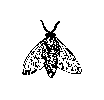
\includegraphics{fly}
\caption{A sample black and white graphic.}
\end{figure}

\begin{figure}
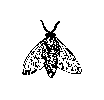
\includegraphics[height=1in, width=1in]{fly}
\caption{A sample black and white graphic
that has been resized with the \texttt{includegraphics} command.}
\end{figure}


As was the case with tables, you may want a figure that spans two
columns.  To do this, and still to ensure proper ``floating''
placement of tables, use the environment \textbf{figure*} to enclose
the figure and its caption.  And don't forget to end the environment
with \textbf{figure*}, not \textbf{figure}!

\begin{figure*}
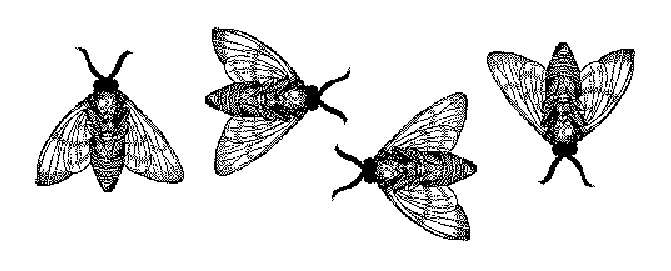
\includegraphics{flies}
\caption{A sample black and white graphic
that needs to span two columns of text.}
\end{figure*}


\begin{figure}
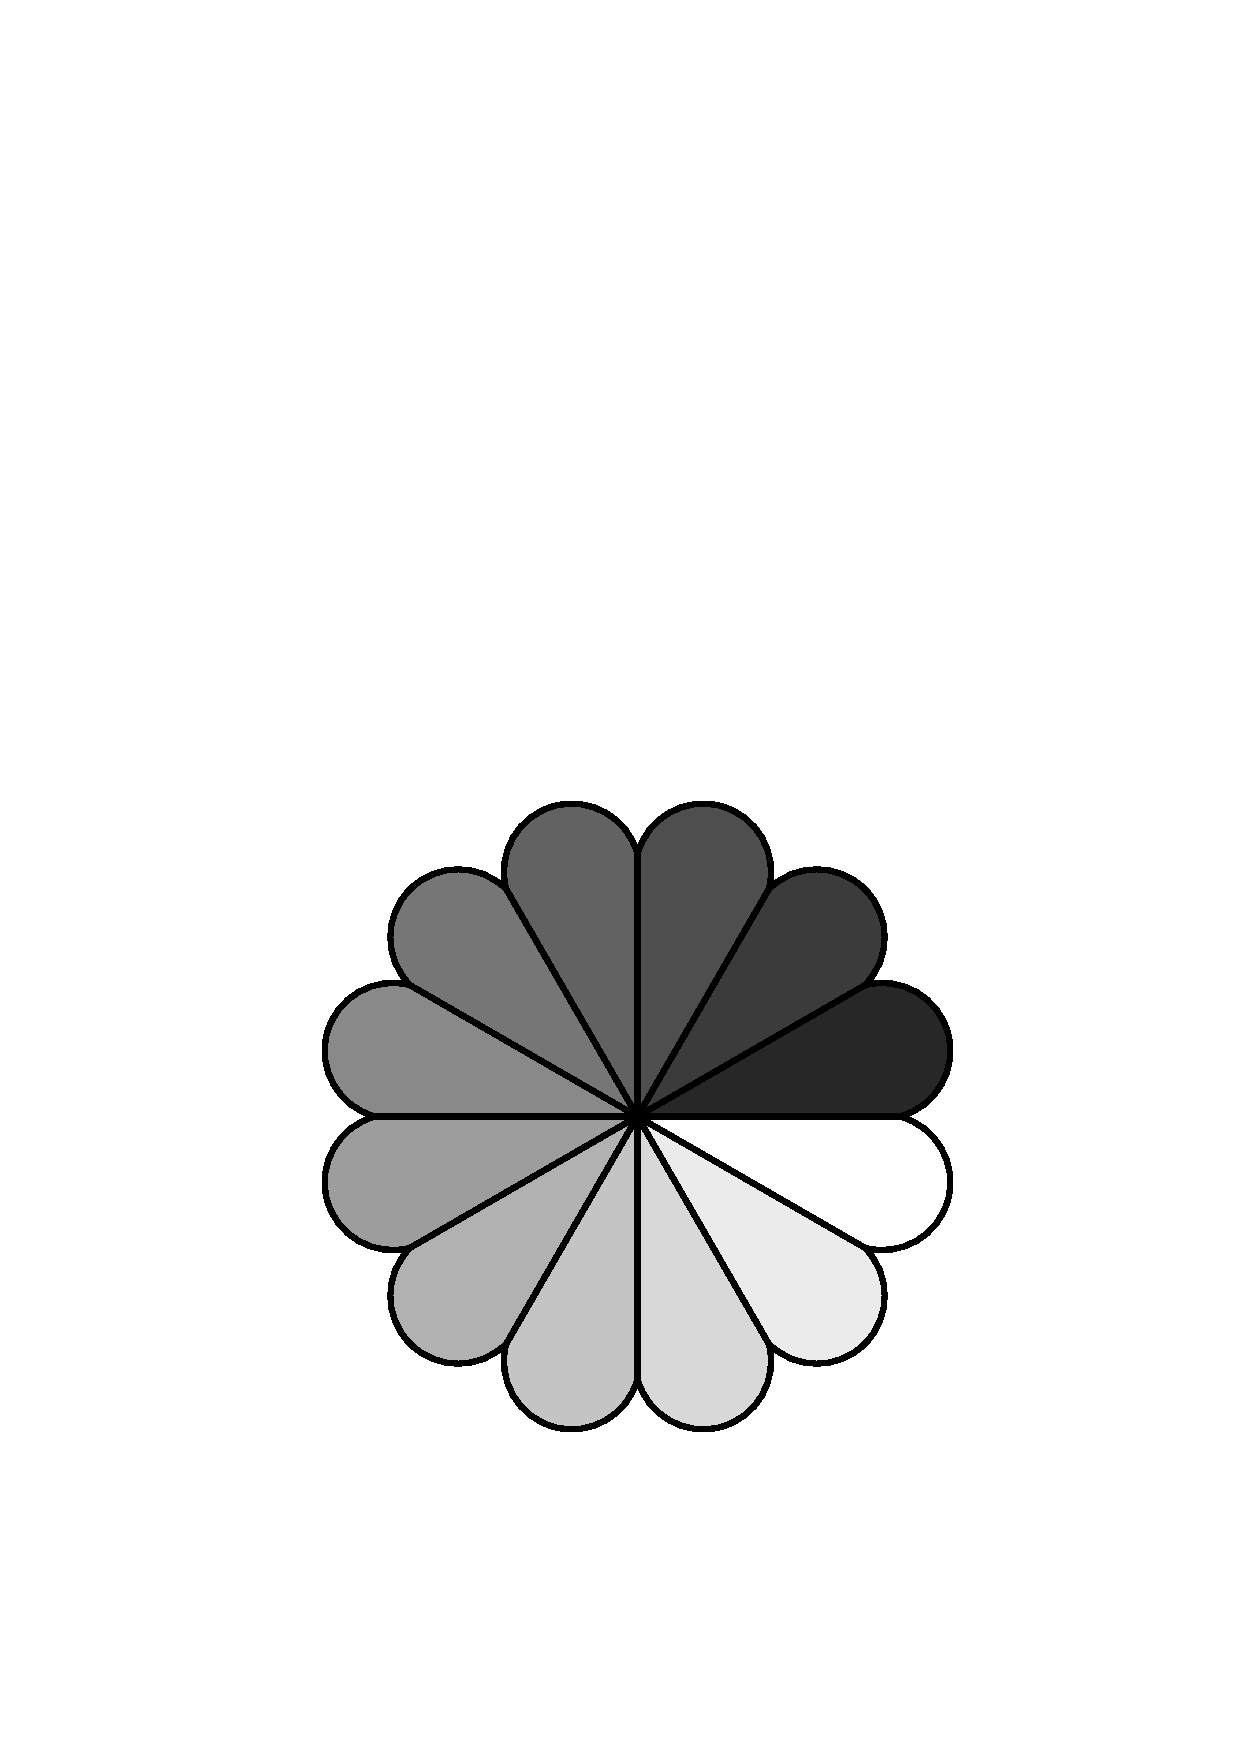
\includegraphics[height=1in, width=1in]{rosette}
\caption{A sample black and white graphic that has
been resized with the \texttt{includegraphics} command.}
\end{figure}

\subsection{Theorem-like Constructs}

Other common constructs that may occur in your article are the forms
for logical constructs like theorems, axioms, corollaries and proofs.
ACM uses two types of these constructs:  theorem-like and
definition-like.

Here is a theorem:
\begin{theorem}
  Let $f$ be continuous on $[a,b]$.  If $G$ is
  an antiderivative for $f$ on $[a,b]$, then
  \begin{displaymath}
    \int^b_af(t)\,dt = G(b) - G(a).
  \end{displaymath}
\end{theorem}

Here is a definition:
\begin{definition}
  If $z$ is irrational, then by $e^z$ we mean the
  unique number that has
  logarithm $z$:
  \begin{displaymath}
    \log e^z = z.
  \end{displaymath}
\end{definition}

The pre-defined theorem-like constructs are \textbf{theorem},
\textbf{conjecture}, \textbf{proposition}, \textbf{lemma} and
\textbf{corollary}.  The pre-defined de\-fi\-ni\-ti\-on-like constructs are
\textbf{example} and \textbf{definition}.  You can add your own
constructs using the \textsl{amsthm} interface~\cite{Amsthm15}.  The
styles used in the \verb|\theoremstyle| command are \textbf{acmplain}
and \textbf{acmdefinition}.

Another construct is \textbf{proof}, for example,

\begin{proof}
  Suppose on the contrary there exists a real number $L$ such that
  \begin{displaymath}
    \lim_{x\rightarrow\infty} \frac{f(x)}{g(x)} = L.
  \end{displaymath}
  Then
  \begin{displaymath}
    l=\lim_{x\rightarrow c} f(x)
    = \lim_{x\rightarrow c}
    \left[ g{x} \cdot \frac{f(x)}{g(x)} \right ]
    = \lim_{x\rightarrow c} g(x) \cdot \lim_{x\rightarrow c}
    \frac{f(x)}{g(x)} = 0\cdot L = 0,
  \end{displaymath}
  which contradicts our assumption that $l\neq 0$.
\end{proof}

\section{Conclusions}
This paragraph will end the body of this sample document.
Remember that you might still have Acknowledgments or
Appendices; brief samples of these
follow.  There is still the Bibliography to deal with; and
we will make a disclaimer about that here: with the exception
of the reference to the \LaTeX\ book, the citations in
this paper are to articles which have nothing to
do with the present subject and are used as
examples only.
%\end{document}  % This is where a 'short' article might terminate



\appendix
%Appendix A
\section{Headings in Appendices}
The rules about hierarchical headings discussed above for
the body of the article are different in the appendices.
In the \textbf{appendix} environment, the command
\textbf{section} is used to
indicate the start of each Appendix, with alphabetic order
designation (i.e., the first is A, the second B, etc.) and
a title (if you include one).  So, if you need
hierarchical structure
\textit{within} an Appendix, start with \textbf{subsection} as the
highest level. Here is an outline of the body of this
document in Appendix-appropriate form:
\subsection{Introduction}
\subsection{The Body of the Paper}
\subsubsection{Type Changes and  Special Characters}
\subsubsection{Math Equations}
\paragraph{Inline (In-text) Equations}
\paragraph{Display Equations}
\subsubsection{Citations}
\subsubsection{Tables}
\subsubsection{Figures}
\subsubsection{Theorem-like Constructs}
\subsubsection*{A Caveat for the \TeX\ Expert}
\subsection{Conclusions}
\subsection{References}
Generated by bibtex from your \texttt{.bib} file.  Run latex,
then bibtex, then latex twice (to resolve references)
to create the \texttt{.bbl} file.  Insert that \texttt{.bbl}
file into the \texttt{.tex} source file and comment out
the command \texttt{{\char'134}thebibliography}.
% This next section command marks the start of
% Appendix B, and does not continue the present hierarchy
\section{More Help for the Hardy}

Of course, reading the source code is always useful.  The file
\path{acmart.pdf} contains both the user guide and the commented
code.

\begin{acks}
  The authors would like to thank Dr. Yuhua Li for providing the
  matlab code of  the \textit{BEPS} method. 

  The authors would also like to thank the anonymous referees for
  their valuable comments and helpful suggestions. The work is
  supported by the \grantsponsor{GS501100001809}{National Natural
    Science Foundation of
    China}{http://dx.doi.org/10.13039/501100001809} under Grant
  No.:~\grantnum{GS501100001809}{61273304}
  and~\grantnum[http://www.nnsf.cn/youngscientsts]{GS501100001809}{Young
    Scientsts' Support Program}.

\end{acks}
